\documentclass[12pt]{extarticle}
\usepackage{tempora}
\usepackage[T1, T2A]{fontenc}
\usepackage[utf8]{inputenc}
\usepackage[english, ukrainian]{babel}
\usepackage{geometry}
\usepackage{graphicx}
\usepackage{multirow}
\usepackage{multicol}
\usepackage{float}
\graphicspath{{/home/artem/Pictures}}
\geometry
{
    a4paper,
    left=30mm,
    top=15mm,
    right=20mm,
    bottom=15mm,
}

\begin{document}
\begin{titlepage}
    \begin{center}
        \textbf{\normalsize{\MakeUppercase{
            Міністерство Освіти і науки України
            Національний університет "Львівська політехніка"
        }}}

        \begin{flushright}
        \textbf{ІКНІ}\\
        Кафедра \textbf{ПЗ}
        \end{flushright}
        \vspace{15mm}

        \includegraphics[width=0.4\textwidth]{lpnu_logo.png}

        \vspace*{\fill}

        \textbf{\normalsize{\MakeUppercase{Звіт}}}
            
        До лабораторної роботи №9

        \textbf{на тему:} “Бінарний пошук в упорядкованому масиві.”

        \textbf{з дисципліни:} "Алгоритми і структури даних”
            
        \vspace*{\fill}

        \begin{flushright}

            \textbf{Лектор:}\\
            доцент кафедри ПЗ\\
            Коротєєва Т. О.\\
            \vspace{12pt}

            \textbf{Виконав:}\\
            студент групи ПЗ-24\\
            Губик А. С.\\
            \vspace{12pt}

            \textbf{Прийняв:}\\
            асистент кафедри ПЗ\\
            Вишневський К. О.\\
        \vspace{12pt}
        \end{flushright}

        Львів -- 2023
            
            
    \end{center}
\end{titlepage}

\subsection*{Тема роботи} 
Бінарний пошук в упорядкованому масиві.

\subsection*{Мета роботи} Навчитися застосовувати алгоритм бінарного пошуку при розв’язуванні задач та перевірити його ефективність на різних масивах даних. Експериментально визначити складність алгоритму.

\subsection*{Індивідуальне завдання}
Варіант 3: Дано одновимірний масив цілих чисел A[і], де і =1,2,…,n. Визначити елемент, що є меншим від максимального на 5. Скільки разів він зустрічається у даному масиві та порядковий номер його першого входження. Вивести кількість порівнянь.

\subsection*{Теоретичні відомості}
Бінарним називають таке 2-арне дерево, в якого один потомок є лівим, а другий - правим. Вершина бінарного дерева може взагалі не мати потомків, або мати тільки ліве, або тільки праве піддерево, або обидва піддерева одночасно.

Рівнем або рангом вершини по відношенню до дерева називають довжину шляху від кореня до цієї вершини. Довжина шляху - це кількість дуг, які треба пройти від кореня для досягнення даної вершини.

Висота дерева дорівнює кількості рівнів у дереві.

Бінарне дерево з m вершинами називають збалансованим, якщо різниця між рівнями будь-яких двох вершин не більша від одиниці.

Алгоритми обходу дерева

Алгоритм обходу дерева являє собою спосіб методичного дослідження вершин дерева, при якому кожна вершина проглядається тільки один раз. Повне проходження дерева дає лінійне розміщення вершин, після якого можна говорите про "наступну вершину" як таку, що розміщується або перед даною вершиною, або після неї. Розглянемо три алгоритми обходу бінарного дерева на прикладі дерева, зображеного на рис. 1, а.

Бінарний, або двійковий пошук – алгоритм пошуку елементу у відсортованому масиві. Це класичний алгоритм, ще відомий як метод дихотомії (ділення навпіл).

Якщо елементи масиву впорядковані, задача пошуку суттєво спрощується. Згадайте, наприклад, як Ви шукаєте слово у словнику. Стандартний метод пошуку в упорядкованому масиві – це метод поділу відрізка навпіл, причому відрізком є відрізок індексів 1..n. Дійсно, нехай масив A впорядкований за зростанням і m (k < m < l) – деякий індекс. Нехай Buffer = A[m]. Тоді якщо Buffer > b, далі елемент необхідно шукати на відрізку k..m-1, а якщо Buffer < b – на відрізку m+1..l.

Для того, щоб збалансувати кількість обчислень в тому і іншому випадку, індекс m необхідно обирати так, щоб довжина відрізків k..m, m..l була (приблизно) рівною. Описану стратегію пошуку називають бінарним пошуком.

b – елемент, місце якого необхідно знайти. Крок бінарного пошуку полягає у порівнянні шуканого елемента з середнім елементом Buffer = A[m] в діапазоні пошуку [k..l]. Алгоритм закінчує роботу при Buffer = b (тоді m – шуканий індекс). Якщо Buffer > b, пошук продовжується ліворуч від m, а якщо Buffer < b – праворуч від m. При l < k пошук закінчується, і елемент не знайдено.
\subsection*{Вихідний код}

{\fontfamily{pcr}\selectfont
\begin{verbatim}
    #include <iostream>
    #include <vector>
    #include <algorithm>
    #include <cstdlib>  
    #include <ctime>
    
    int iter = 0;
    
    int binarySearch(const std::vector<int>& arr, int target) {
        int left = 0;
        int right = arr.size() - 1;
    
        while (left <= right) {
            ++iter;
            int mid = left + (right - left) / 2;
    
            if (arr[mid] == target) {
                return mid;
            }
            else if (arr[mid] < target) {
                left = mid + 1; 
                std::cout << "\nПошук в:\n";
                for (int i = left; i <= right; i++)
                {
                    std::cout << arr[i] << " ";
                }
                std::cout << std::endl;
            }
            else {
                right = mid - 1; 
                std::cout << "\nПошук в:\n";
                for (int i = left; i <= right; i++)
                {
                    std::cout << arr[i] << " ";
                }
                std::cout << std::endl;
            }
        }
    
        return -1; 
    }
    
    int main()
    {
        setlocale(LC_CTYPE, "ukr");
        int n;
        std::cout << "Введiть розмiр масиву: ";
        std::cin >> n;
    
        std::vector<int> A(n);
    
        std::srand(static_cast<unsigned int>(std::time(0)));
    
        for (int i = 0; i < n; ++i) {
            A[i] = rand() % 100; 
        }
    
        std::cout << "\nМасив перед операцiями:\n";
        for (int elem : A) {
            std::cout << elem << " ";
        }
        std::cout << std::endl;
    
    
        std::sort(A.begin(), A.end());
        auto maxIt = std::max_element(A.begin(), A.end());
    
        std::cout << "\nМасив після сортування:\n";
        for (int elem : A) {
            std::cout << elem << " ";
        }
        std::cout << std::endl;
    
        int k = *maxIt - 5;
        int result = binarySearch(A, k);
    
        if (result != -1) {
            std::cout << "\nЕлемент " << k << " знайдено пiд iндексом " << result << ".\n";
        }
        else {
            std::cout << "\nЕлемент " << k << " не знайдено в масивi.\n";
        }
    
        std::cout << "\nКiлькiсть порiвнянь: " << iter;
    }
\end{verbatim}
}
\vspace{12pt}
\begin{figure}[H]
    \centering
    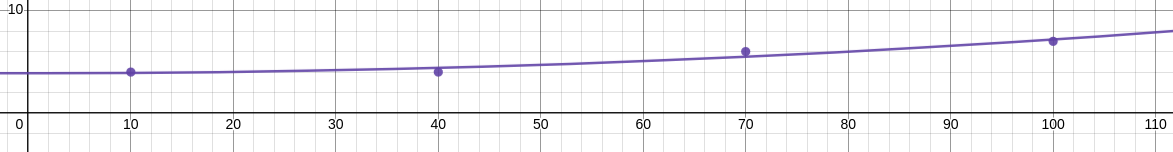
\includegraphics[width=0.90\textwidth]{graph.png}
    \caption{}
\end{figure}
\begin{figure}[H]
    \centering
    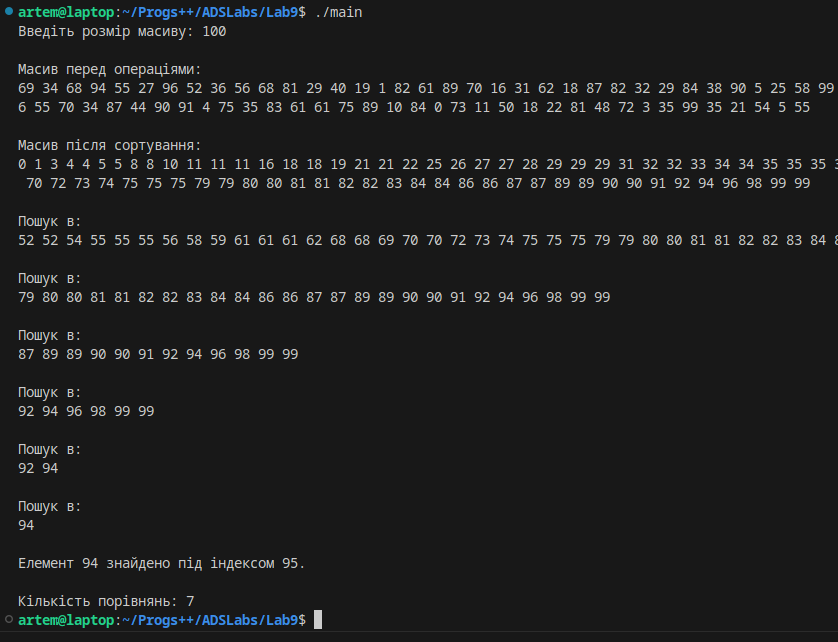
\includegraphics[width=0.90\textwidth]{log.png}
    \caption{}
\end{figure}

\subsection*{Висновок} 
Бінарний пошук є найшвидшим агоритмом пошуку, але при цьому потребу сортування масиву.
\end{document}
